\documentclass{article}

\usepackage{graphicx}
\usepackage{indentfirst}
\usepackage[a4paper, total={6in, 8in}]{geometry}
\usepackage{hyperref}
\usepackage{fancyhdr}
\usepackage{listings}
\usepackage{xepersian}
\settextfont{XB Zar.ttf}
\setlatintextfont{Times New Roman.ttf}

\begin{document}


%title page%
\begin{titlepage}
	\begin{center}
		\vspace{0.2cm}
		
		
\includegraphics[width=0.4\textwidth]{sharif.png}\\
		\vspace{0.2cm}
		\textbf{ \Huge{آزمایش شماره 3}}\\
		\vspace{0.25cm}
		\textbf{ \Large{آز شبکه - دکتر بردیا صفایی}}
		\vspace{0.2cm}
		
		
		\large \textbf{دانشکده مهندسی کامپیوتر}\\\vspace{0.1cm}
		\large   دانشگاه صنعتی شریف\\\vspace{0.2cm}
		\large   ﻧﯿﻢ‌سال اول ۰۱-۰۲ \\\vspace{0.10cm}
		\large{\href{mailto:mehrshad.mirmohammadi@gmail.com}{مهرشاد میرمحمدی - 98109634}}\\
		\large{\href{mailto:parhaamsaremi@gmail.com}{پرهام صارمی - 97101959}}\\
		\large{\href{mailto:mofayezi.m@gmail.com}{محمدرضا مفیضی - 98106059}}\\
	\end{center}
\end{titlepage}
%title page%

\newpage

%pages header
\pagestyle{fancy}
\fancyhf{}
\fancyfoot{}
\setlength{\headheight}{59pt}
\cfoot{\thepage}
\lhead{آزمایش شماره 3}
\rhead{
\includegraphics[width=0.1\textwidth]{sharif.png}\\
		دانشکده مهندسی کامپیوتر
}
\chead{آز شبکه}
%pages header
\section{wireshark}
\subsection{بدست‌آوردن captcha}

همانند دستور عمل می‌کنیم، با این تفاوت که به جای استفاده ازهمانند دستور عمل می‌کنیم، با این تفاوت که به جای استفاده از SSL ، از TLS استفاده می‌کنیم. دلیل آن هم این است که SSL منسوخ شده و TLS جای آن را گرفته است. همچنین این پروتکل در ورژن wireshark مورد استفاده موجود نبود. لیست فایل‌‌های استخراج شده و captchaی بدست‌آمده را می‌توان در تصاویر \ref{fig:1} و \ref{fig:captcha} دید.

\begin{figure}[h!]
	\centering
	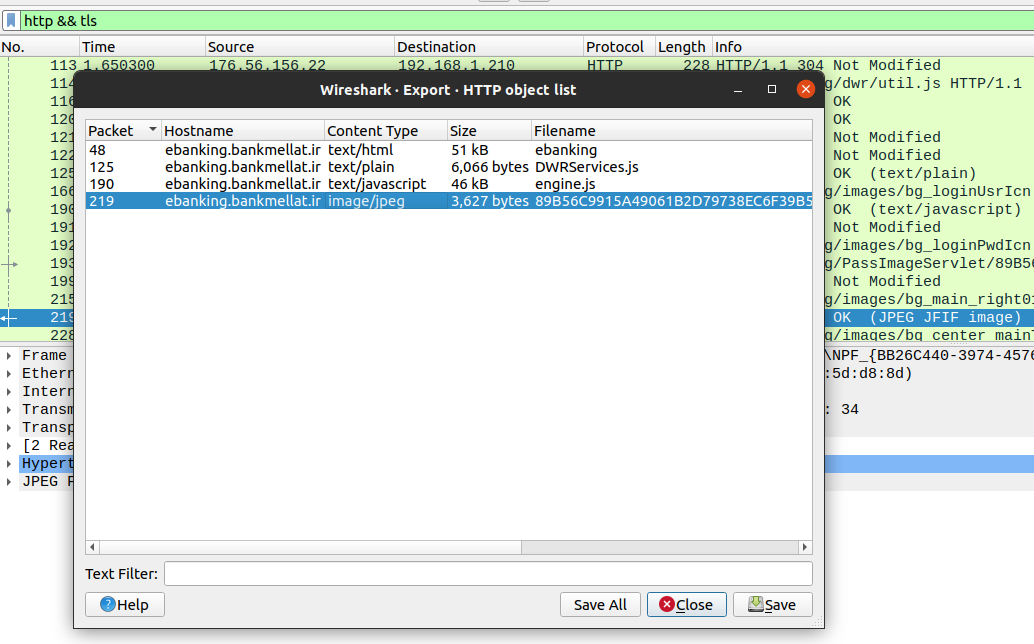
\includegraphics[width=0.9\textwidth]{src/1.png}
	\caption{پنجره‌ی ذخیره‌سازی فایل‌های بدست‌آمده.}
	\label{fig:1}
\end{figure}
\begin{figure}[h!]
	\centering
	
\includegraphics[width=0.5\textwidth]{src/captcha.jpeg}
	\caption{عکس بدست‌آمده.}
	\label{fig:captcha}
\end{figure}

\subsection{سوال‌ها}
\begin{enumerate}
    \item {
    این اطلاعات و آماره‌‌ها را می‌توان از طریق منو‌ی statistics موجود در wireshark بدست آورد. برای مثال با استفاده از بخش سلسله مراتب پروتکل‌ها می‌توان دید پروتکل‌های استفاده شده کدام‌‌ها هستند، از هر کدام چند پکت موجود است و چند درصد از پکت‌ها و بایت‌ها برای آن بوده است. تصویر \ref{fig:2} نمونه خروجی این ابزار است. همچنین با استفاده از باقی ابزار‌‌ها می‌توان اطلاعات دیگری همانند طول بسته‌ها، ترافیک و تعداد بسته‌های بین بخش‌های مختلف شبکه، زمان بین پاسخ‌ها و … بدست‌آورد.
    \begin{figure}[h!]
    	\centering
    	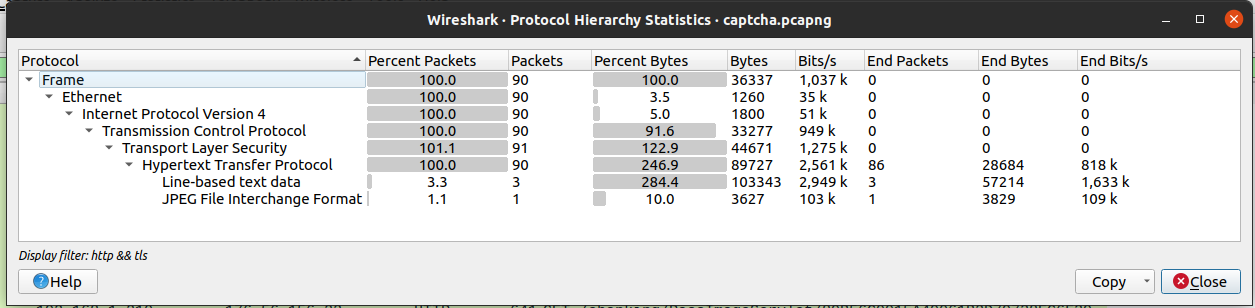
\includegraphics[width=0.9\textwidth]{src/2.png}
    	\caption{statistics > Protocols Hierarchy}
    	\label{fig:2}
    \end{figure}
    }
    \item {
    پروتکل RTP یک پروتکل بیدرنگ برای انتقال صدا و تصویر در شبکه‌ها با بستر IP است. این پروتکل معمولا بر پایه‌ی UDP است و برای streaming استفاده می‌شود. همچنین معمولا برای کنترل ترتیب رسیدن بسته‌ها، از پرتوکل RTCP هم به همراه آن استفاده می‌شود.
    
    در wireshark می‌توان با رفتن به Teⅼephony سپس RTP و سپس RTP streams اطالعات مربوط به آن را یافت. اطلاعاتی مانند آدرس و پورت مبدا و مقصد، میانگین و حداکثر jitter ، گمشدگی و …‬ که در تصویر \ref{fig:3} هم می‌توان دید. همچنین امکان ضبط و بخش محتوا به صورت مستقیم هم موجود است.
    \begin{figure}[h!]
    	\centering
    	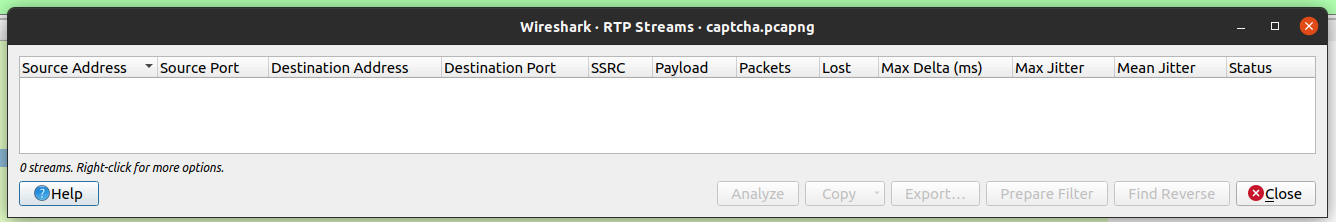
\includegraphics[width=0.9\textwidth]{src/3.png}
    	\caption{‫‪Telephony‬‬ ‫>‬ ‫‪RTP‬‬ ‫>‬ ‫‪RTP‬‬ ‫‪Streams}
    	\label{fig:3}
    \end{figure}
    }
\end{enumerate}

\section{DNS}
ابتدا bind9 را همانند تصویر \ref{fig:4} نصب می‌کنیم. ما از 
\lr{ubuntu 20.04} 
استفاده می‌کنیم.

\begin{figure}[h!]
	\centering
	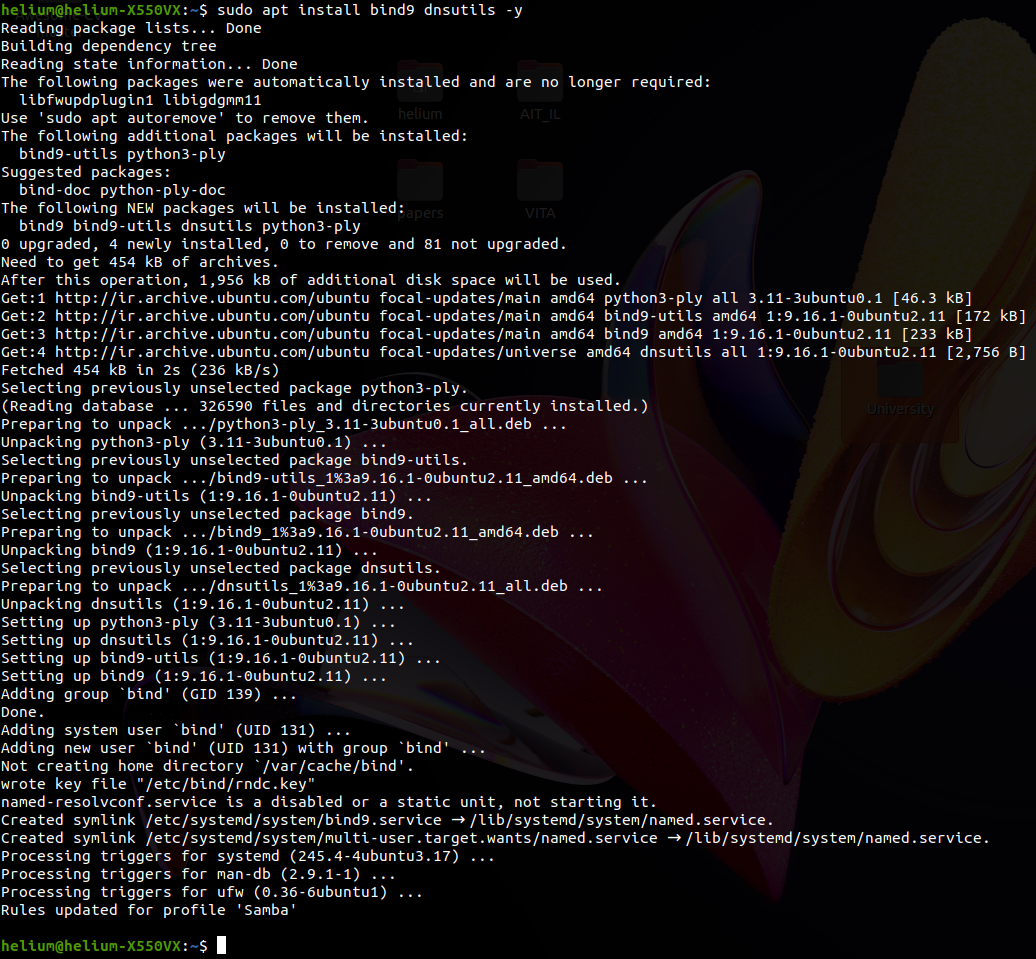
\includegraphics[width=0.9\textwidth]{src/4.png}
	\caption{}
	\label{fig:4}
\end{figure}

مطابق شکل \ref{fig:5} یک منطقه با عنوان \lr{NetLab8.edu} ایجاد می‌کنیم. (عدد ۸ شماره‌ی گروه است.)

\begin{figure}[h!]
	\centering
	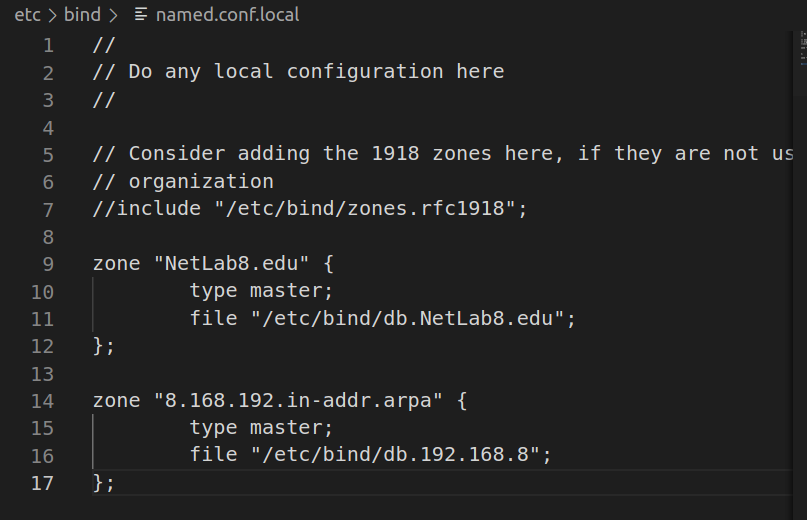
\includegraphics[width=0.9\textwidth]{src/5.png}
	\caption{}
	\label{fig:5}
\end{figure}

فایل 
\lr{/etc/bind/db.NetLab8.edu }
مطابق تصویر \ref{fig:6} پر می‌کنیم. همانطور که در تصویر مشخص است یک nameserver با نام 
\lr{ns.NetLab8.edu}
 و ip با مقدار 1.8.168.192 ایجاد می‌کنیم. به دامنه‌ی سرور آدرس 2.8.168.192 اختصاص می‌دهیم. دو زیر دامنه‌ی 
\lr{group1.NetLab8.edu} و \lr{group2.NetLab8.edu }
را به ترتیب در ip های 
3.8.168.192 و
4.8.168.192 و با نام‌های مستعار 
\lr{cNameGroup1.NetLab8.edu} و 
\lr{cNameGroup2.NetLab8.edu } 
تعریف می‌کنیم.
\begin{figure}[h!]
	\centering
	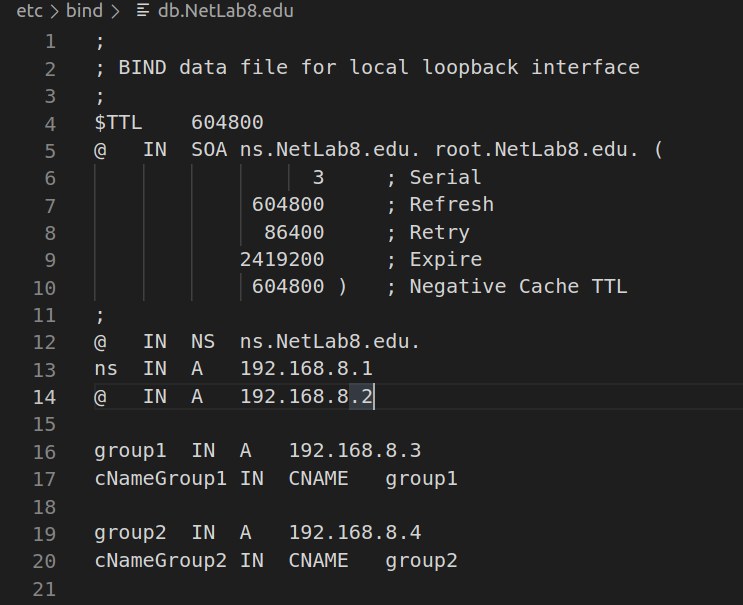
\includegraphics[width=0.9\textwidth]{src/6.png}
	\caption{}
	\label{fig:6}
\end{figure}

مطابق تصویر \ref{fig:7} تنظمیات رکورد‌های معکوس را هم در فایل 
\lr{/etc/bind/db.192.168.8} قرار می‌دهیم.

\begin{figure}[h!]
	\centering
	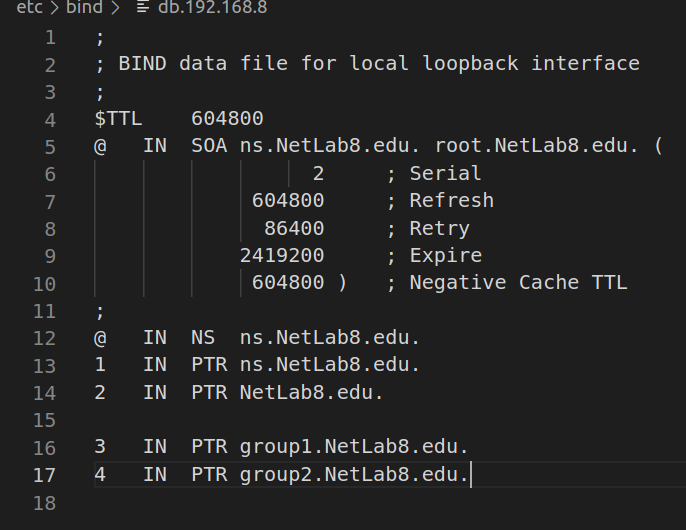
\includegraphics[width=0.9\textwidth]{src/7.png}
	\caption{}
	\label{fig:7}
\end{figure}

فایل 
\lr{/etc/resolvconf/resolv.conf.d/head} 
را مطابق تصویر \ref{fig:8} پر می‌کنیم.

\begin{figure}[h!]
	\centering
	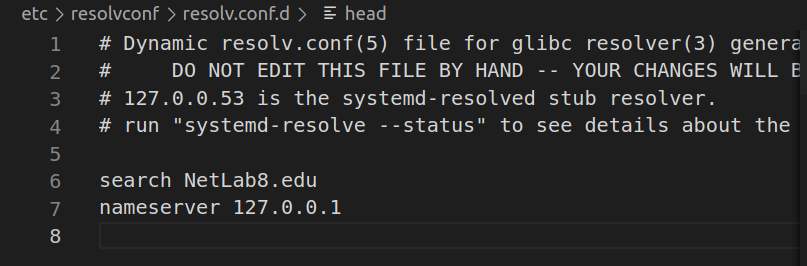
\includegraphics[width=0.9\textwidth]{src/8.png}
	\caption{}
	\label{fig:8}
\end{figure}

سپس دستور‌های زیر را به ترتیب اجرا می‌کنیم تا \lr{bind9} مجددا راه‌اندازی شده و آدرس سرور ما قبل از همه‌ی سرویس‌دهنده‌های مورد اعتماد سیستم قرار بگیرد. سپس با استفاده با دستور \lr{nslookup} از درستی کارکرد سرور DNS اطمینان حاصل می‌کنیم. (مطابق تصاویر \ref{fig:9} و \ref{fig:10})
\begin{latin}
	\begin{lstlisting}
sudo systemctl restart bind9
sudo named-checkconf
sudo resolvconf -u
	\end{lstlisting}
\end{latin}

\begin{figure}[h!]
	\centering
	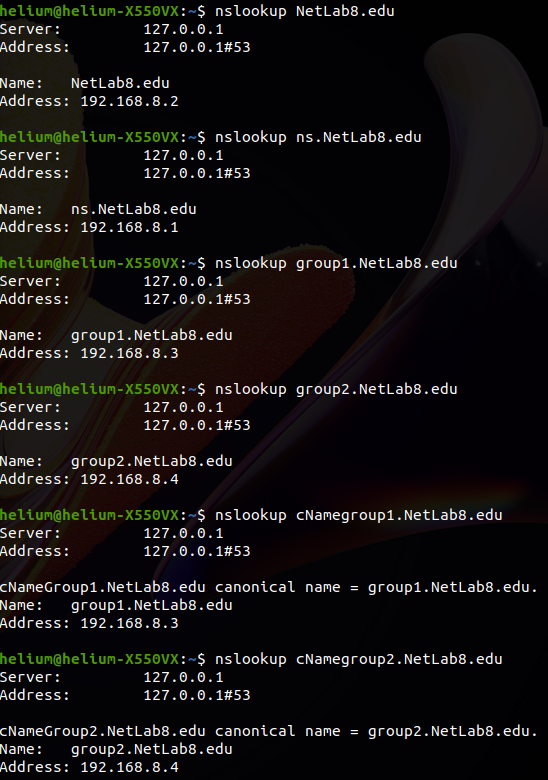
\includegraphics[width=0.9\textwidth]{src/9.png}
	\caption{}
	\label{fig:9}
\end{figure}
\begin{figure}[h!]
	\centering
	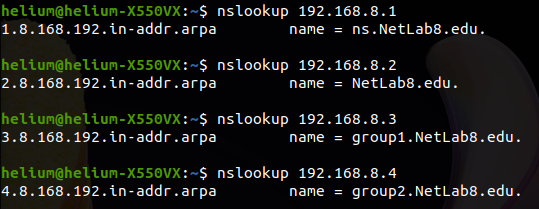
\includegraphics[width=0.9\textwidth]{src/10.png}
	\caption{}
	\label{fig:10}
\end{figure}

\subsection{سوالات}
\begin{enumerate}
	\item 
	اطلاعات پکت‌های DNS رد و بدل شده برای بدست آوردن ip متعلق به \lr{group2.NetLab8.edu } و نام متعلق به آدرس 3.8.168.192 را با استفاده از وایرشارک capture می‌کنیم. در تصویر \ref{fig:11} و \ref{fig:12} پرس‌ و جو و پاسخ سرور را به ترتیب مشاهده می‌کنیم.
	\item 
	همانطور که در تصاویر هم می‌توانیم ببینیم، نوع پرس و جوی اول از نوع A و نوع پرس و جوی دوم از نوع PTR است.
\end{enumerate}

\begin{figure}[h!]
	\centering
	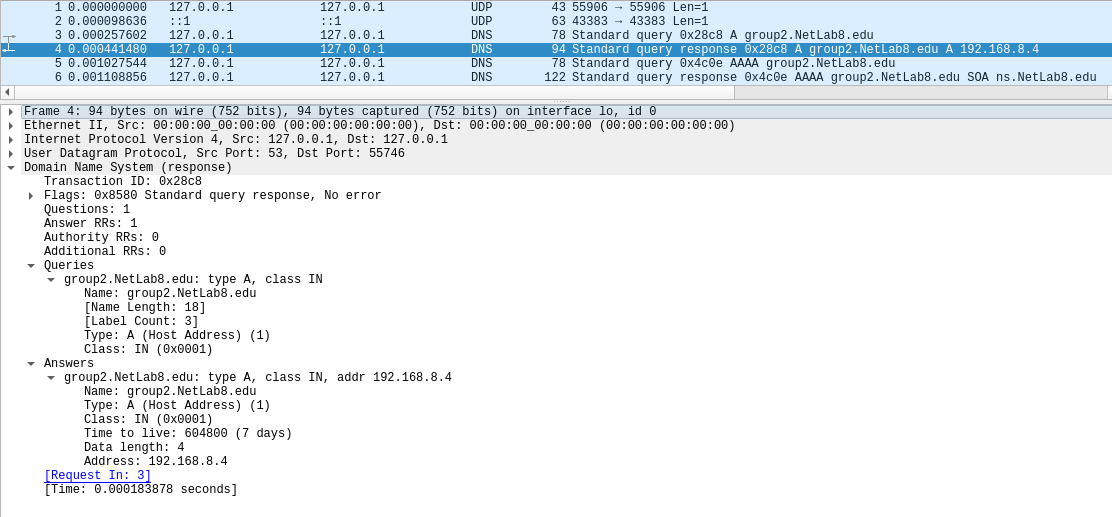
\includegraphics[width=0.9\textwidth]{src/11.png}
	\caption{}
	\label{fig:11}
\end{figure}
\begin{figure}[h!]
	\centering
	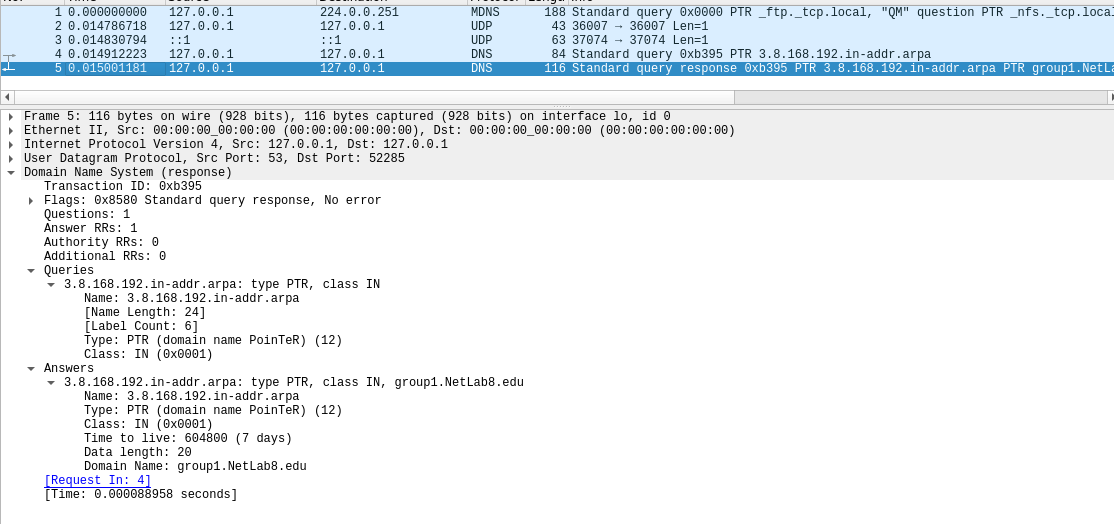
\includegraphics[width=0.9\textwidth]{src/12.png}
	\caption{}
	\label{fig:12}
\end{figure}
\end{document}
